
% Q16
\question The height and the base radius of a right circular cone are $12\text{ cm}$ and $9\text{ cm}$ respectively. The figure shows a frustum which is made by cutting off the upper part of the circular cone. The height of the frustum is $8\text{ cm}$ . Find the volume of the frustum.

\begin{minipage}{0.45\textwidth}
\begin{choices}
    \choice $210\pi\text{ cm}^3$
    \correctchoice $312\pi\text{ cm}^3$
    \choice $324\pi\text{ cm}^3$
    \choice $936\pi\text{ cm}^3$
\end{choices}
\end{minipage}
\begin{minipage}{0.52\textwidth}
\centering
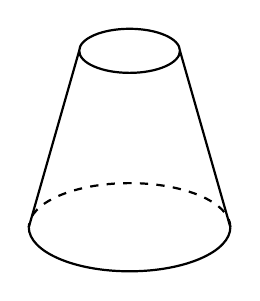
\begin{tikzpicture}[scale=0.8]
    \draw[thick] (-0.8,2.8) ellipse (0.8 and 0.35);
    \draw[thick] (-2.4,0) arc (180:360:1.6 and 0.7);
    \draw[thick,dashed] (0.8,0) arc (0:180:1.6 and 0.7);
    \draw[thick] (-1.6,2.8) -- (-2.4,0);
    \draw[thick] (0,2.8) -- (0.8,0);
\end{tikzpicture}
\end{minipage}
\begin{solution}
The height of the upper cone is $12 - 8 = 4\text{ cm}$, which is $\frac{4}{12} = \frac{1}{3}$ of the original cone's height. \\
Volume of the frustum:
\[ \frac{1}{3}\pi(9)^2(12) \times \left[1 - \left(\frac{1}{3}\right)^3\right] = 324\pi \times \frac{26}{27} = 312\pi\text{ cm}^3 \quad \text{(B)} \]
\end{solution}

% Q17
\question In the figure, $ABCD$ is a parallelogram. $E$ is a point lying on $CD$ such that $DE : EC = 2 : 3$ . $AD$ produced and $BE$ produced meet at $F$ while $AE$ produced and $BC$ produced meet at $G$ . If the area of $\triangle DEF$ is $8\text{ cm}^2$ , then the area of $\triangle CEG$ is

\begin{minipage}{0.45\textwidth}
\begin{choices}
    \choice $12\text{ cm}^2$ .
    \choice $18\text{ cm}^2$ .
    \choice $20\text{ cm}^2$ .
    \correctchoice $27\text{ cm}^2$ .
\end{choices}
\end{minipage}
\begin{minipage}{0.52\textwidth}
\centering
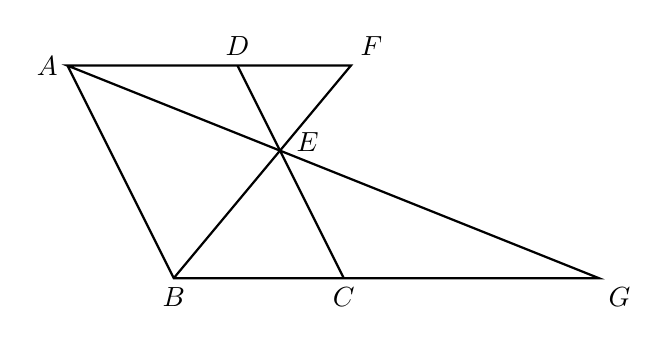
\begin{tikzpicture}[scale=0.9]
    \coordinate (B) at (0,0);
    \coordinate (C) at (2.4,0);
    \coordinate (G) at (6.0,0);
    \coordinate (A) at (-1.5,3.0);
    \coordinate (D) at (0.9,3.0);
    \coordinate (F) at (2.5,3.0);
    \coordinate (E) at (1.5,1.8);
    \draw[thick] (A) -- (B) -- (G) -- (A) -- (F) -- (B);
    \draw[thick] (D) -- (C);
    \node[left] at (A) {$A$};
    \node[below] at (B) {$B$};
    \node[below] at (C) {$C$};
    \node[above] at (D) {$D$};
    \node[right=10pt, above = -4pt] at (E) {$E$};
    \node[above right] at (F) {$F$};
    \node[below right] at (G) {$G$};
\end{tikzpicture}
\end{minipage}
\begin{solution}
Since $\triangle DEF \sim \triangle CEB$ with $DE : EC = 2 : 3$, we have $DF : CB = 2 : 3$, so $DF : DA = 2 : 3$. \\
Thus $\text{Area}(\triangle DEA) = \frac{3}{2} \times \text{Area}(\triangle DEF) = \frac{3}{2}(8) = 12\text{ cm}^2$. \\
Since $\triangle CEG \sim \triangle DEA$ with $EC : ED = 3 : 2$:
\[ \text{Area}(\triangle CEG) = 12 \times \left(\frac{3}{2}\right)^2 = 27\text{ cm}^2 \quad \text{(D)} \]
\end{solution}